В работе был рассмотрен вопрос проектировки беспилотного летательного аппарата (БПЛА), предназаченного для длительного ($\approx24$~часа без дозаправки) в целях мониторинга и разведки. В связи с этим к БПЛА были предъявлены высокие требования по малозаметности и аэродинамическим свойствам. Конструкторами была представлена модель БПЛА, отвечающая требованиям аэродинамики и малозаметности. Вид фюзеляжа представлен на Рис.\ref{fig:BPLA_TSAGI}. 

\begin{figure}[H]
\centering
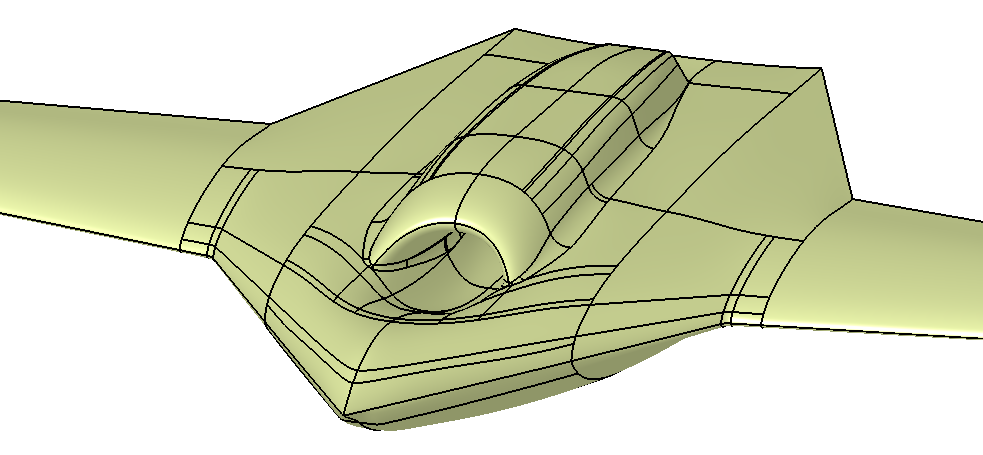
\includegraphics[width=0.6\textwidth]{BPS_Catia}
\caption{вид фюзеляжа БПЛА-ЦАГИ}
\label{fig:BPLA_TSAGI}
\end{figure}

Была поставлена задача построения расчетной модели данного БПЛА и дальнейшего прочностного анализа модели. При построении модели необходимо было учесть дальнейшее возможное изменение формы обводов и, как следствие, изменение аэродинамических нагрузок. Ограничения по режимам полета представлены на Рис.\ref{fig:ModeOfFlight}.
 
\begin{figure}[H]
\begin{subfigure}[b]{0.47\textwidth}
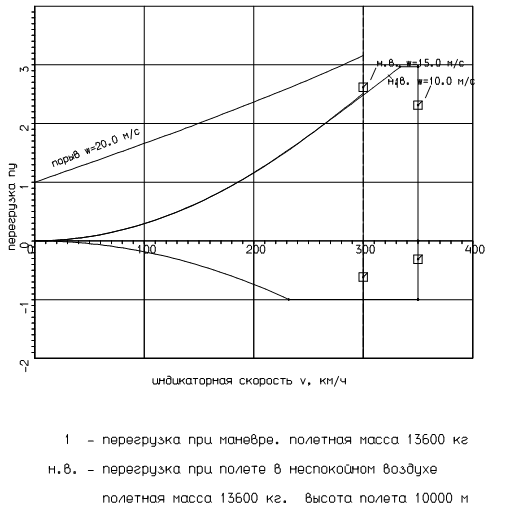
\includegraphics{OverloadGraph}
\label{fig:OverloadGraph}
\end{subfigure}
\begin{subfigure}[b]{0.47\textwidth}
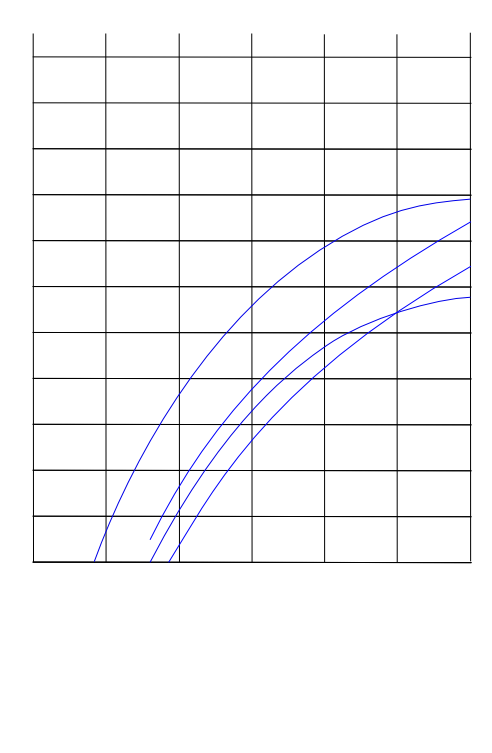
\includegraphics{HeightGraph}
\label{fig:HeightGraph}
\end{subfigure}
\caption{Ограничения на режимы полета}
\label{fig:ModeOfFlight}
\end{figure}

%Не забыть про то, что мы также хотим менять аэродинамику
%Требования: БПЛА, полет на таких-то высотах, столько-то. Весовая сводка такая-то, максимальные перегрузки, коэффициент запаса, аэродинамика. Ограничения - малозаметность, вес, пожаробезопасность отсека двигателя. 
%

